\chapter{Planning and System Design}

\section{Planning and Work Management}
The project was synchronized with GitHub version control from the very beginning. GitHub issues were used to keep track of features that are to be implemented in the project, in addition to patches and fixes. 
\begin{figure}[h]
    \caption{GitHub Issues for Tasks Tracking}
    \centering
    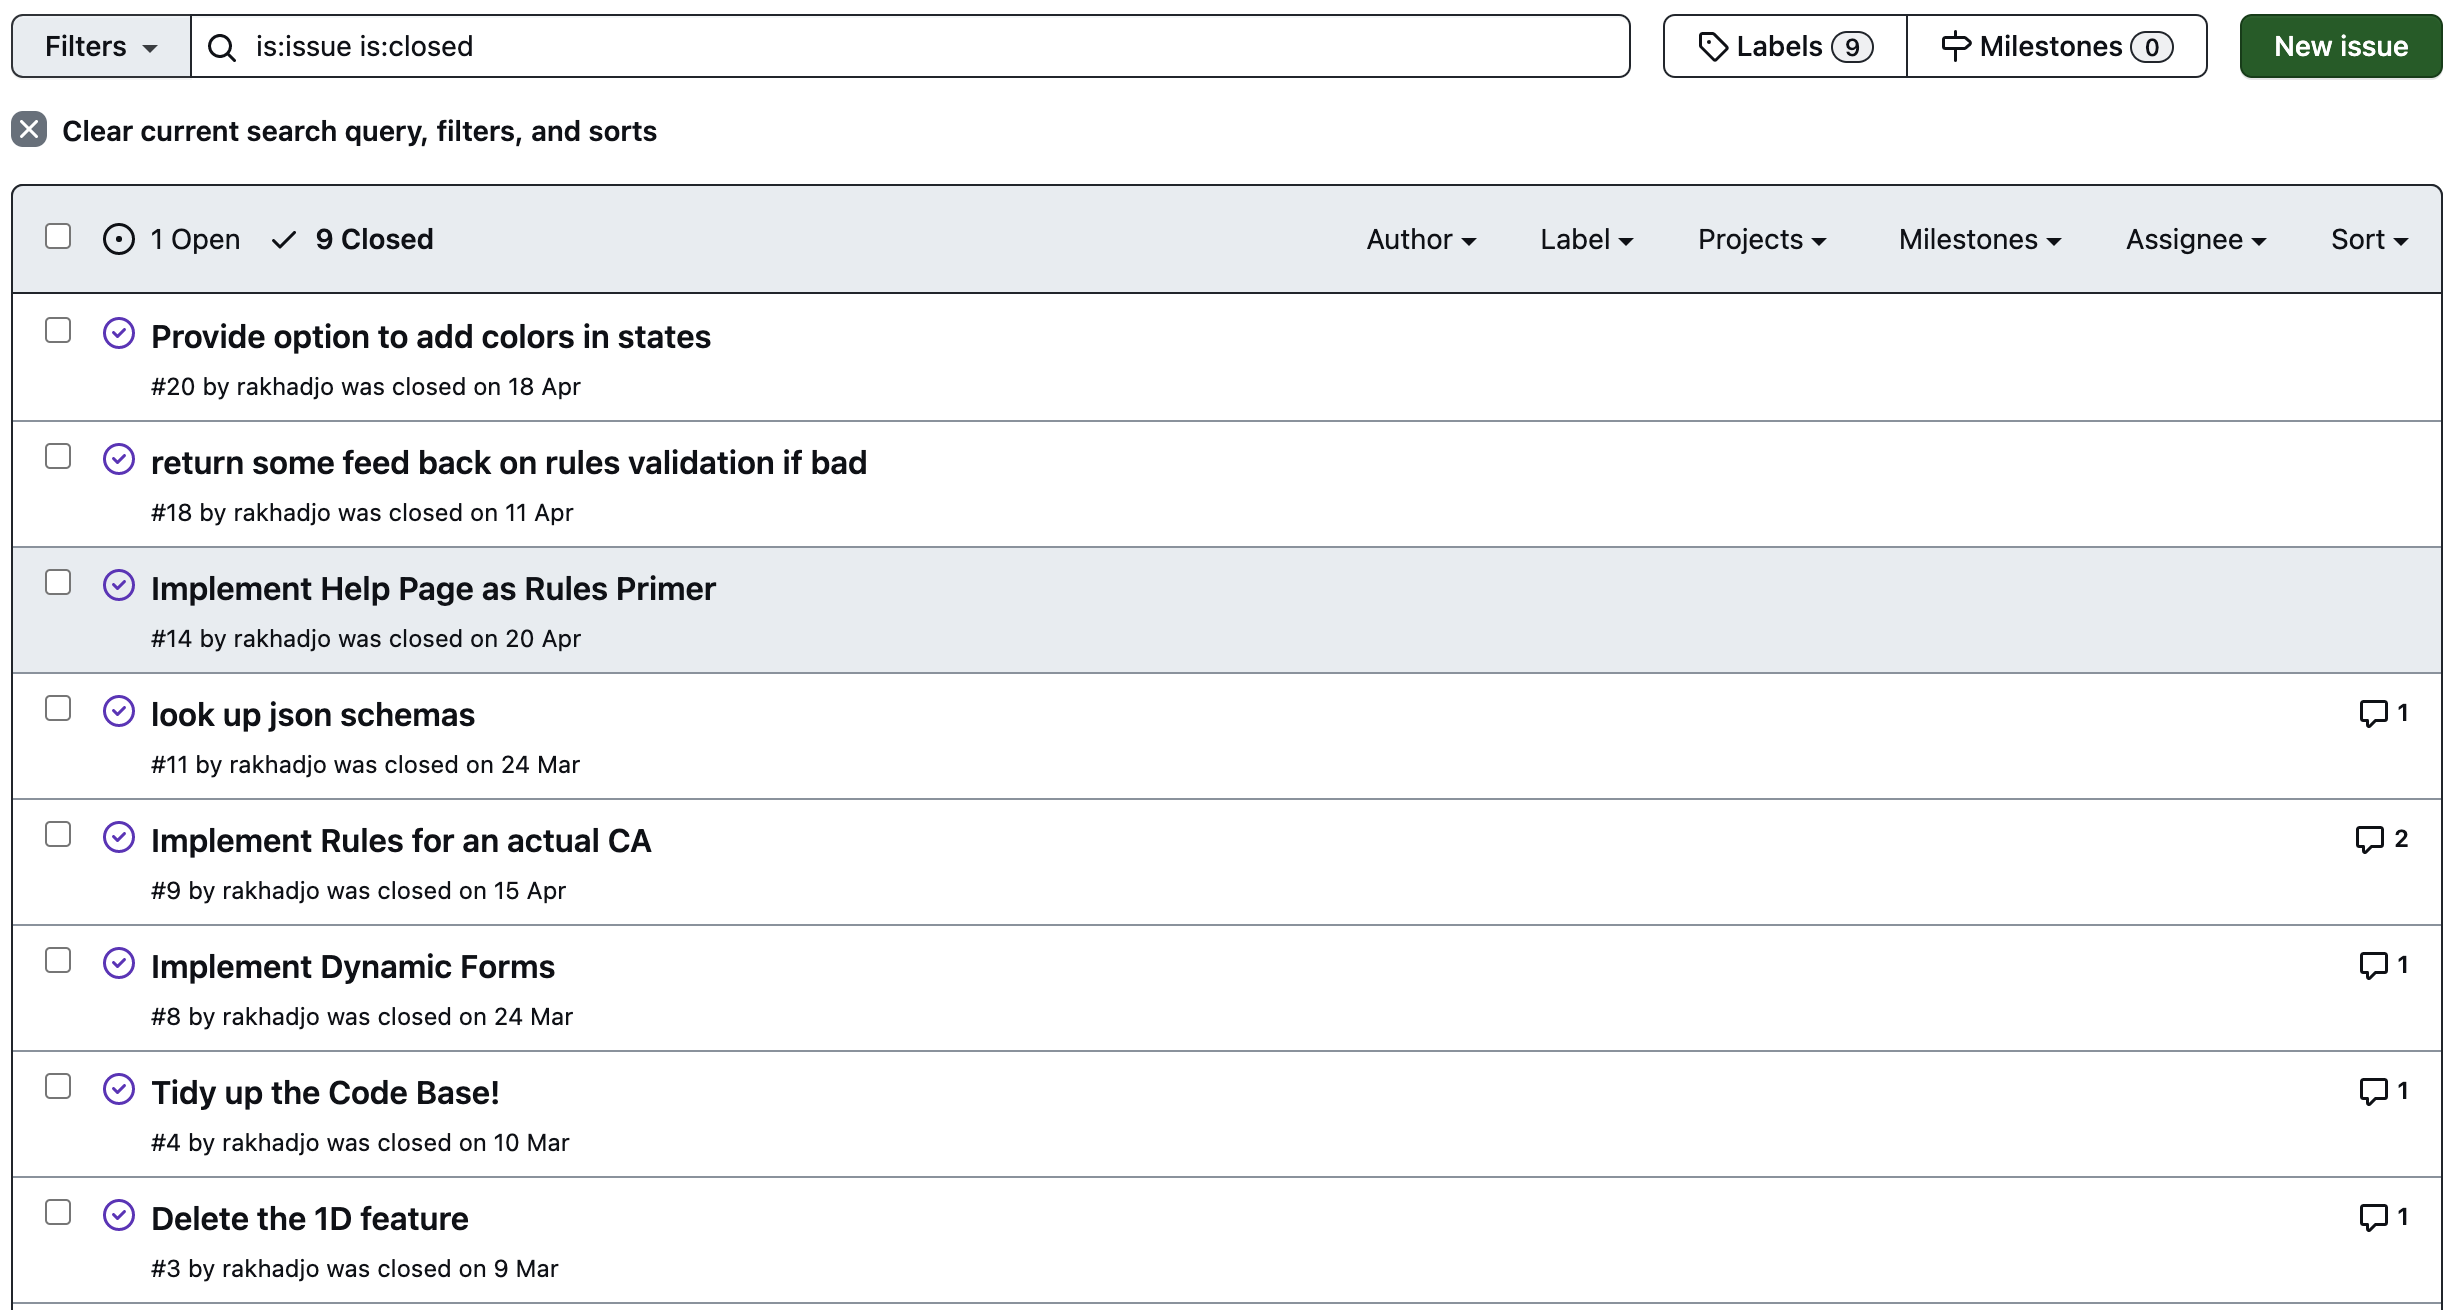
\includegraphics[scale=0.20]{github_issues.png}
\end{figure}
\\ 
Each issue calls for its own feature branch, and each feature is then integrated by merging pull requests from their respective branches to the \texttt{development} branch. \\
\begin{figure}[h]
    \caption{GitHub Pull Requests for Feature Merging}
    \centering
    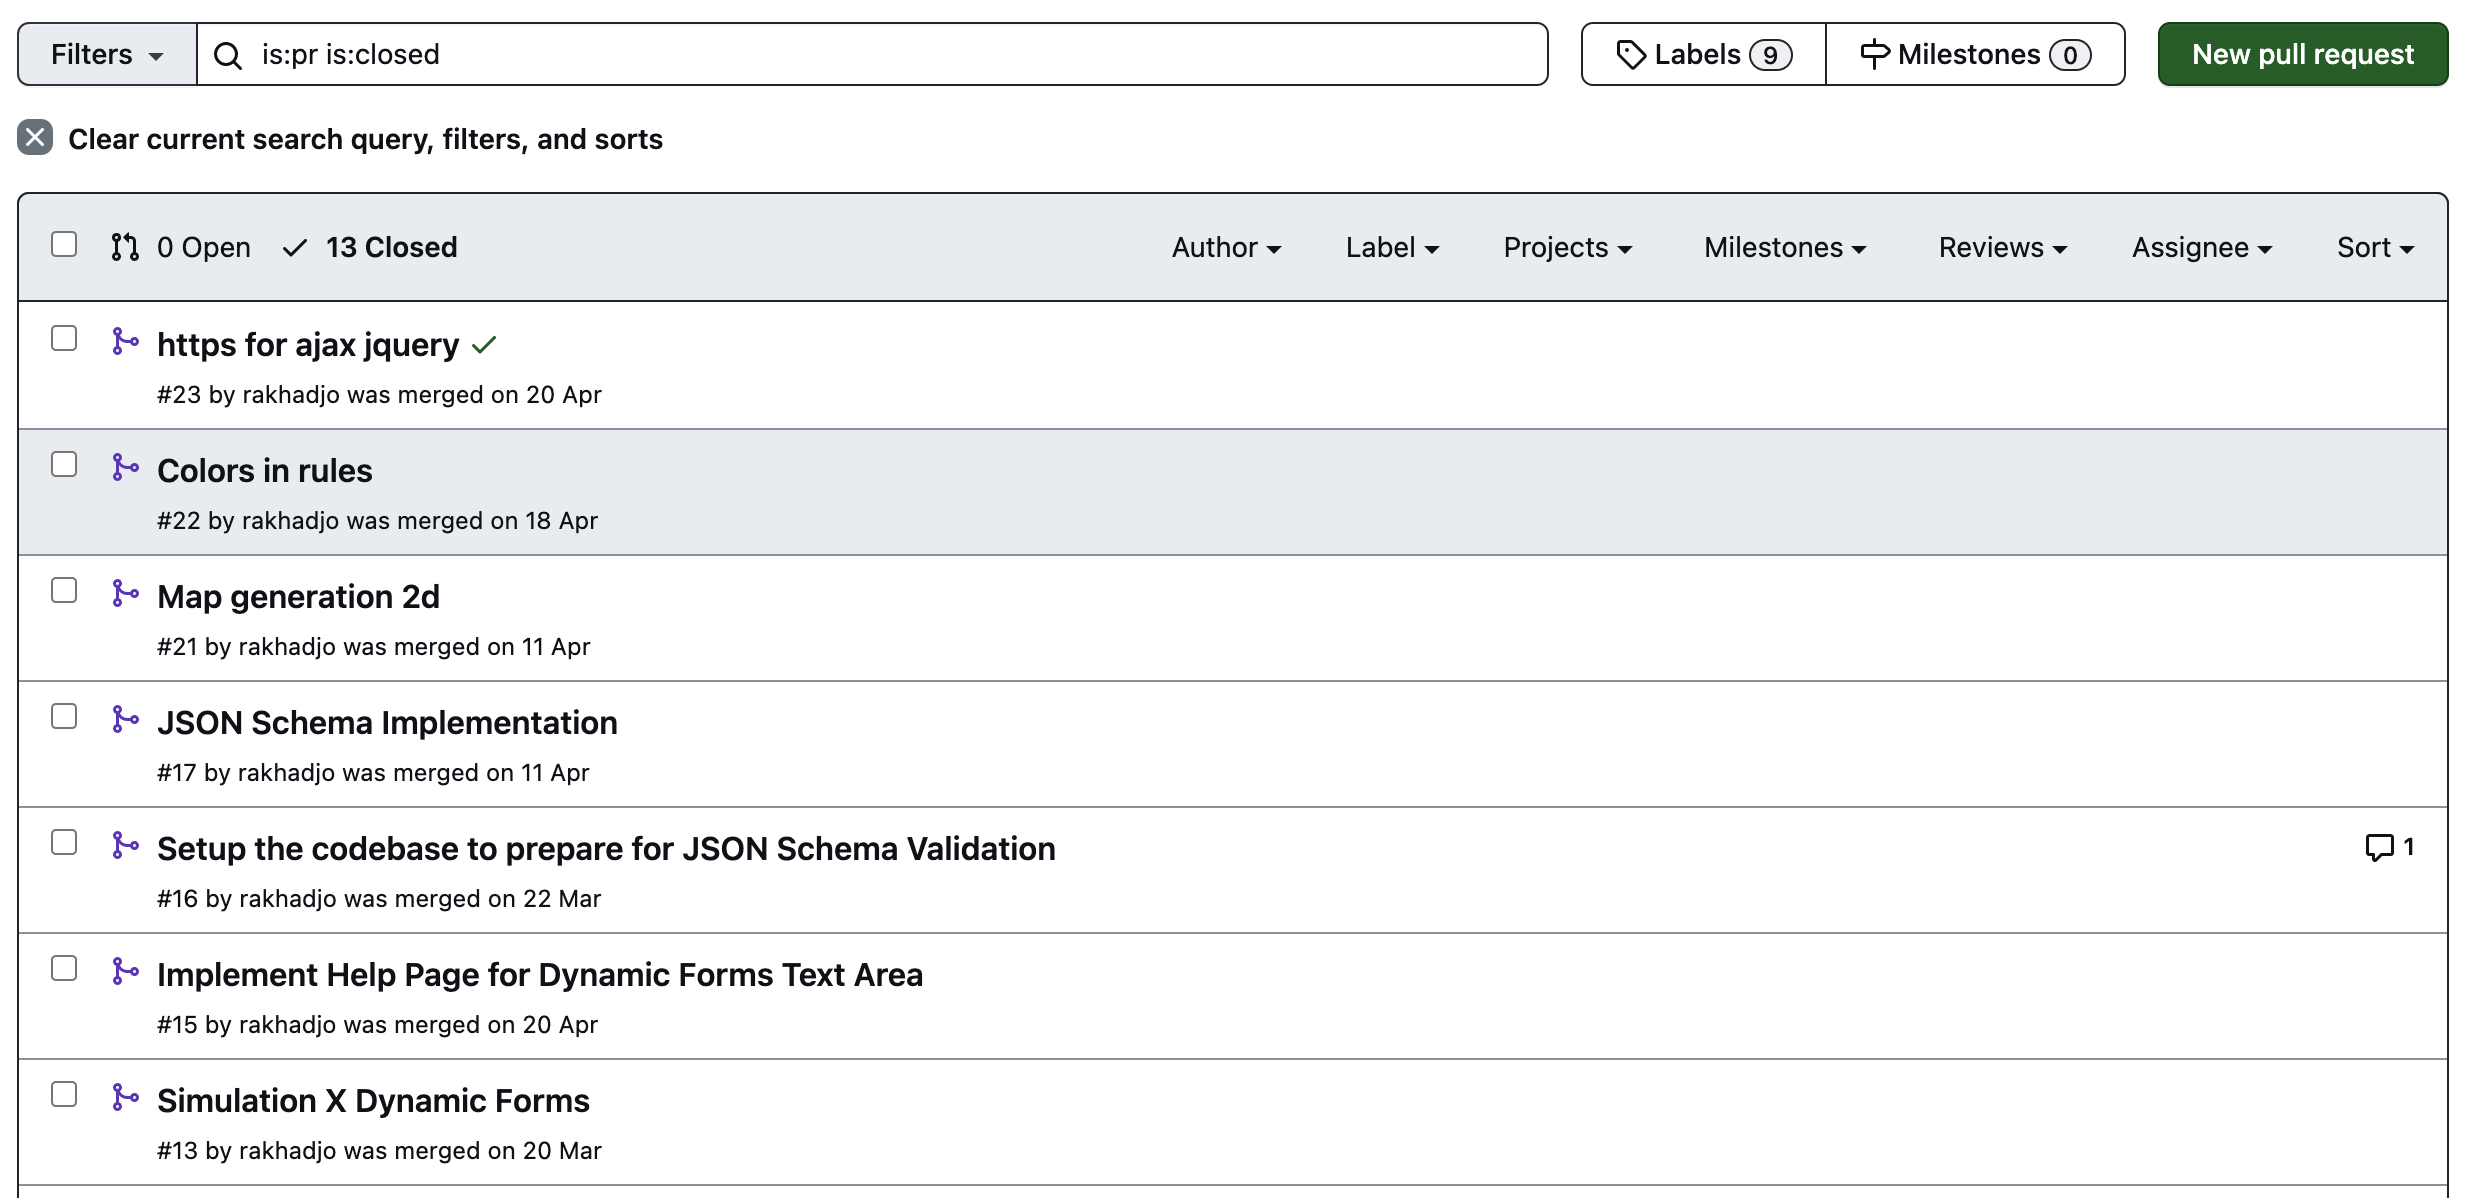
\includegraphics[scale=0.20]{github_prs.png}
\end{figure}
\\ 
A pull request to the \texttt{master} branch from the aforementioned \texttt{development} branch is opened from the very beginning, and merged upon the code freeze for submission.

\section{Features}
The main idea is to create a user interface which should be usable by university students in computer science, with some exposure to Cellular Automata. Note that this project does not aim to introduce the concept of cellular automata to its users. This means that provided the idea of cellular automata and a brief overview of how to use the rules, the user should be able to manipulate the rules and use the simulator.

\subsection{Functional Requirements}
Functional requirements outline the bare minimum as to how the system should behave. This project requires the system to, at the bare minimum and for all kinds of CAs:
\begin{itemize}
    \item \textbf{Graphical User Interface}: The GUI will take inspiration from an IDE, and be as ergonomic as possible.
    \item \textbf{Modify the CA rules}: Editable through the Rule Editor on the left hand side of the GUI. 
    \item \textbf{Change any of the state's colors}: This will be done by modifying the rules' contents in the \texttt{\$\_meta} tag, for preference or real-world visualization.
    \item \textbf{Change the CA rules}: Using the rules' contents from the text editor. 
    \item \textbf{Parse and Validate JSON Rules}: Potentially TV4/JSON Schema implementation.
    \item \textbf{Count Neighbours of Each Individual Cell}: CAs determine next state based on neighbour's states. 
    \item \textbf{Determine next state}: Provided the rules and the neighbour stats. 
\end{itemize}

\subsection{Non-Functional Features}
Non-functional features outline how the system is meant to behave, while describing its limits in its functionality. In the context of this project, the non-functional features are as follows:
\begin{itemize}
    \item \textbf{24/7 Availability}: Hosted on an always-on system.
    \item \textbf{Platform Independence}: Hosted on GitHub Pages, accessible and usable to everyone on the internet.
\end{itemize}

\section{Language Selection}
Due to the time constraint in the project, the final software was written in HTML and JavaScript. This allows the project to be instantly deployed as a static web page during testing, in addition to providing instant availability to the project only through a web browser without any unnecessary downloads.
\\ \\
Java and JavaFX was considered at one point, but JavaFX support online was relatively minimal. Additionally, different versions Java installations wouldn't have given the final project the same level of flexibility in deployment. Installation would therefore be impractical. 
\\ \\
Despite the tech stack being entirely front-end, I am defining the term "front end" as code that functions to change the user interface, and "back end" as code whose functions are not directly seen.

\section{Architectural Diagram}
As the details of each components and micro-components are discussed in the sections following, the below diagram represents the general architectural flow, alongside the names of the components. 
\begin{figure}[H]
    \caption{Architectural Diagram}
    \centering
    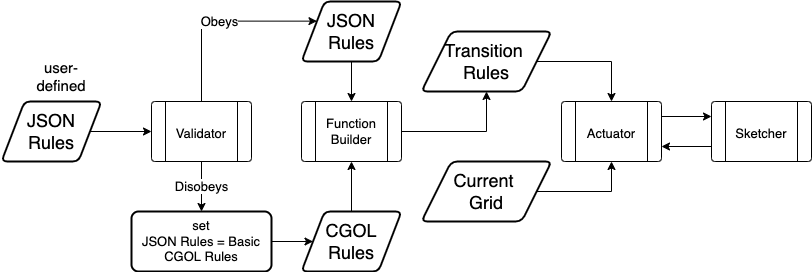
\includegraphics[scale=0.5]{arch.png}
\end{figure}
\noindent It is important to note that the validator, function builder, actuator and sketcher components are displayed as 'predefined', because its implementation will be shown here soon. 
\\ \\
Some components are not present in the diagram. That is because the dynamic rules format are somewhat related to the Validator, and the GUI overarches everything. 

\section{Architectural Components and Implementation}
The following subsections outline the different components working in tandem to fulfill the described features above, and justifying the decisions that were made. Additionally, the final implementation of each components are described in this section.

\subsection{Graphical User Interface (GUI)} \label{gui_component}
The GUI is designed to hold three main components to the system: the CA simulator, the rules editor, and the control buttons. An early sketch of the GUI is provided below: 
\\
\begin{figure}[H]
    \caption{Early GUI Sketch}
    \centering
    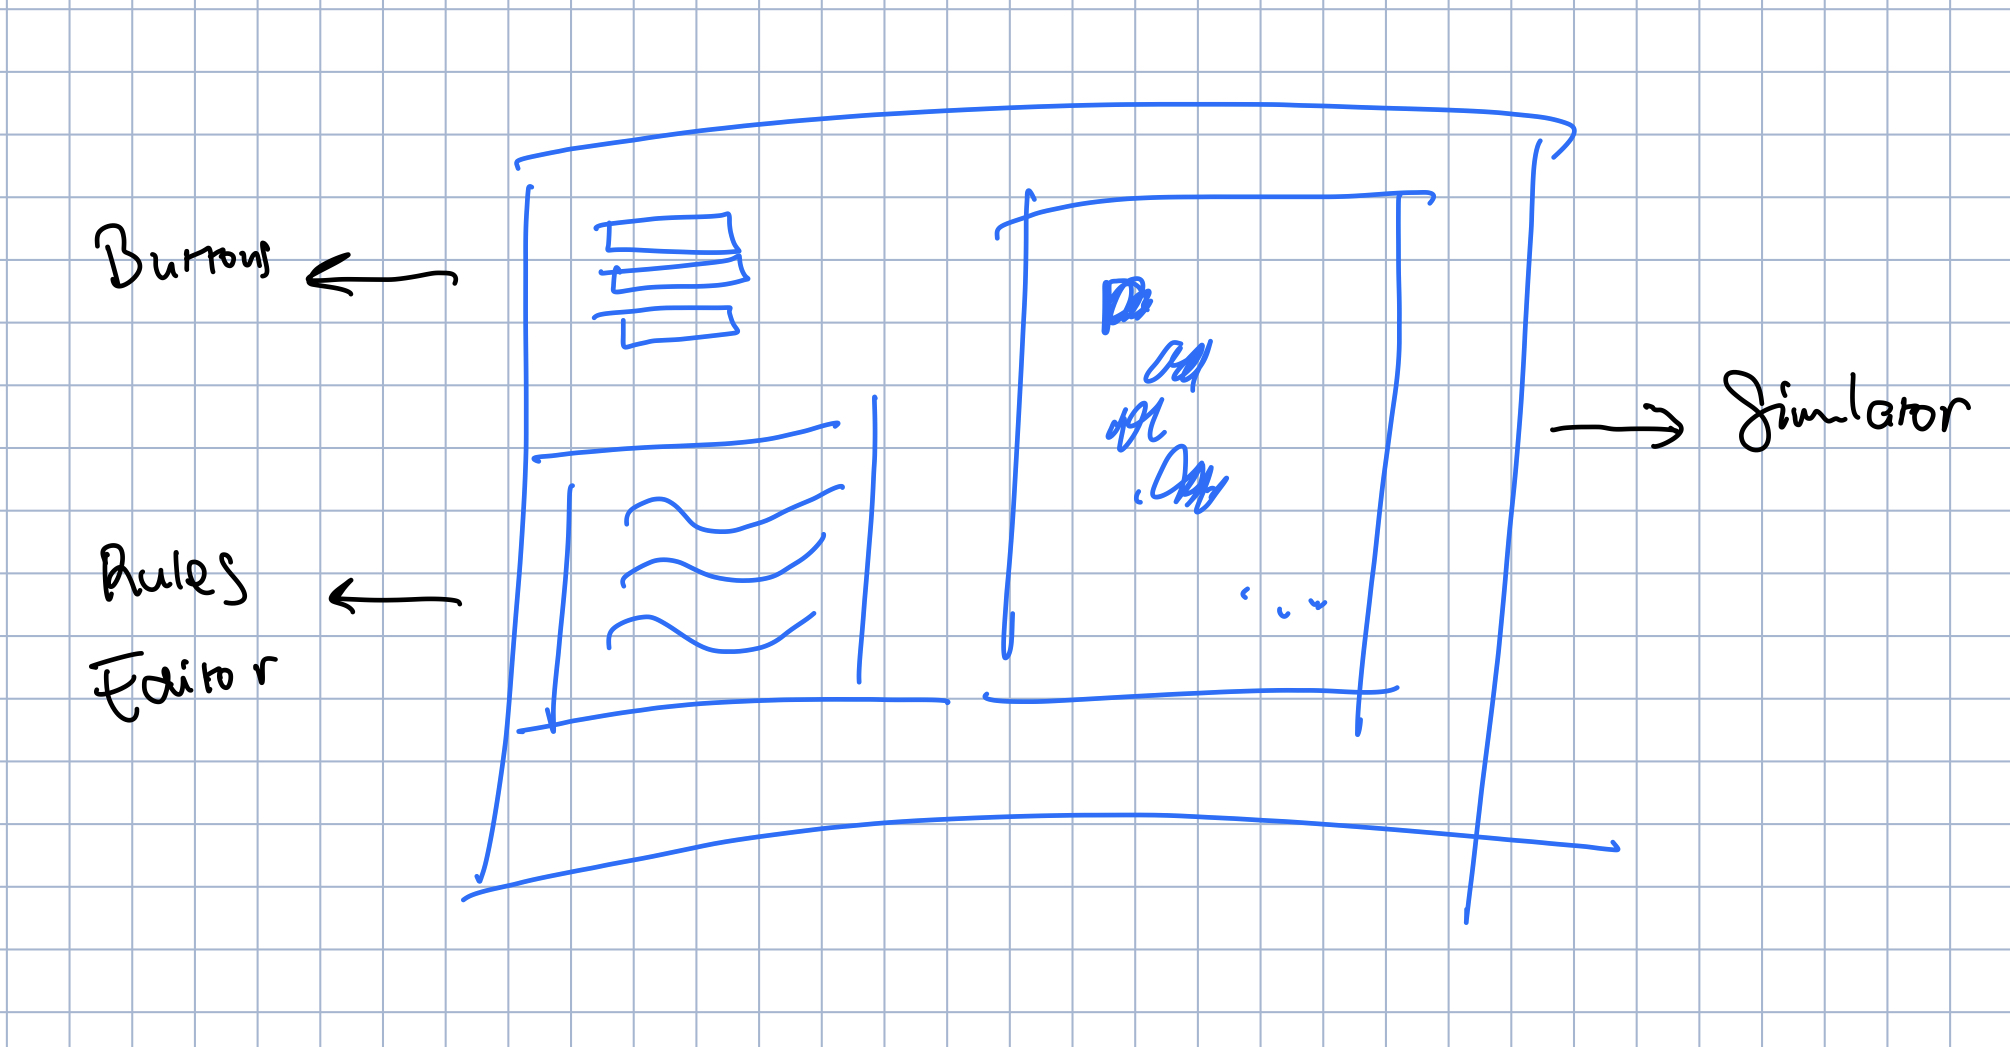
\includegraphics[scale=0.20]{early_ui_mockup.jpeg}
\end{figure}

\noindent The rules editor and buttons are to be positioned on the left side of the screen, whereas the simulator is placed on the right hand side. This design is inspired by a variety of IDEs, where buttons are typically placed on top of the editor area, and the output (in this case the simulator) is positioned on the right (oftentimes bottom). The choice of inspiration from an IDE is that the intended audience (for evaluation) of this project is Computer Science Students. There is a higher chance that the audience has interfaced with an IDE before, and my hypothesis is that this design will increase usability. This IDE-inspired design hopes to be ergonomic by adopting the principle of humans reading from left to right, up to down.
\\ \\
The final GUI is shown in the following:
\\
\begin{figure}[h]
    \caption{Final GUI Design}
    \label{fig:final_gui}
    \centering
    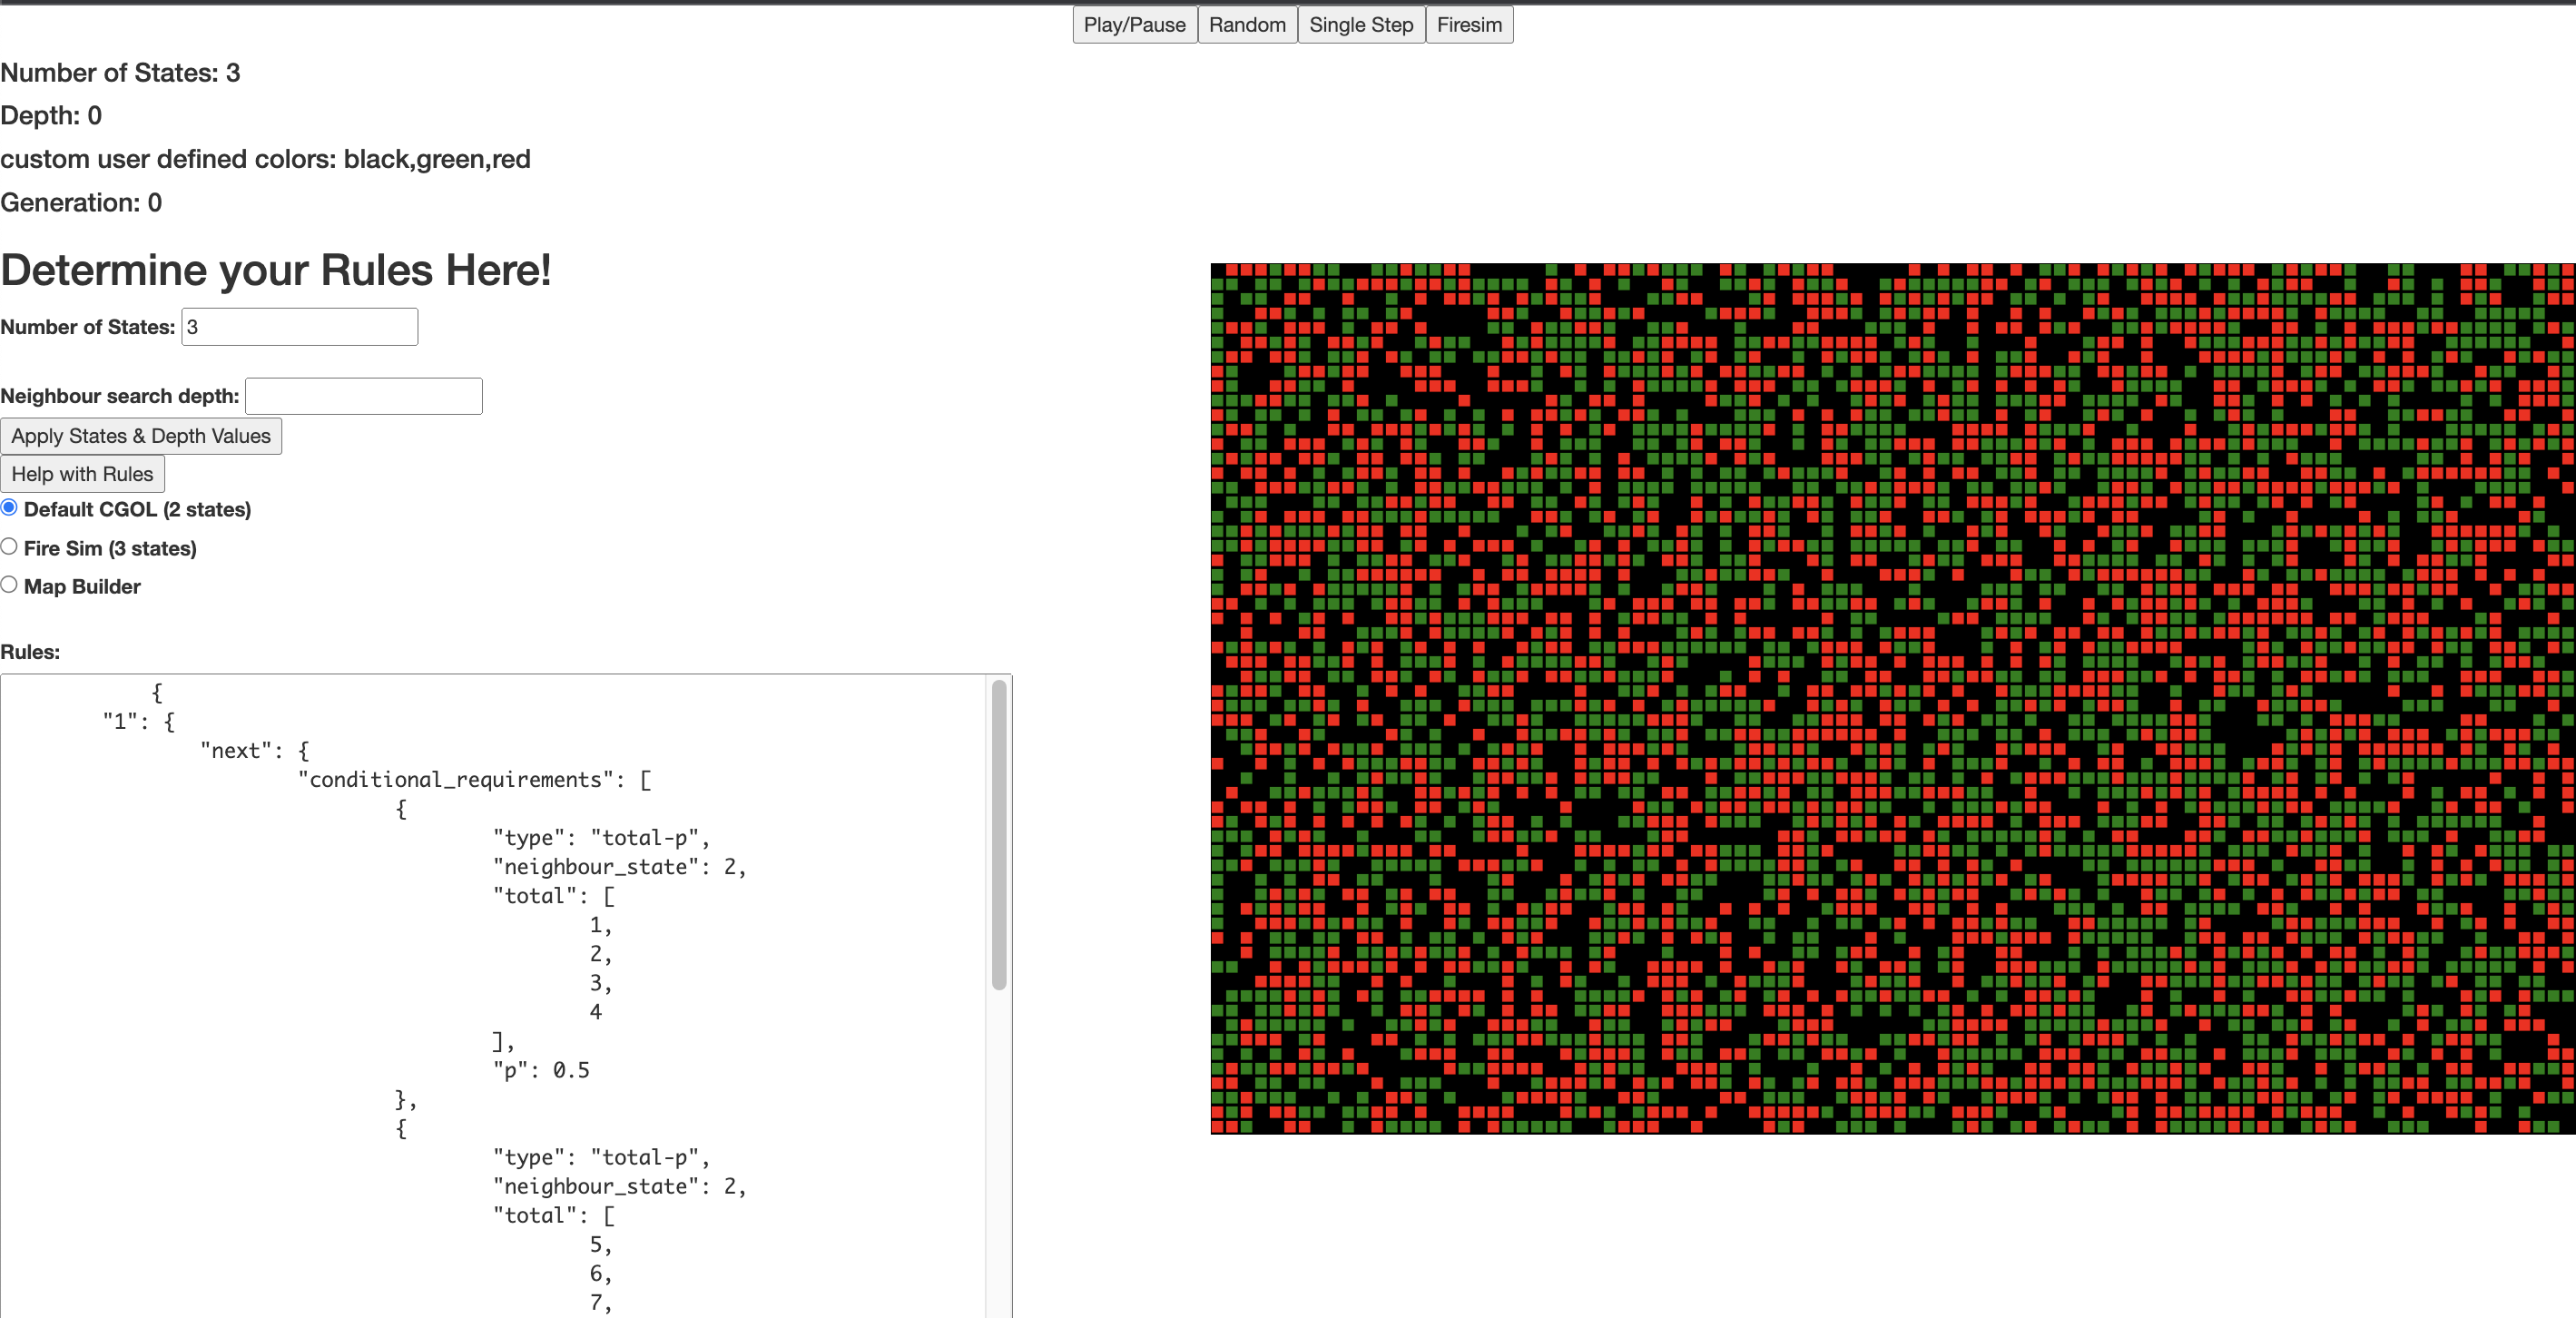
\includegraphics[scale=0.30]{gui_final.png}
\end{figure}
\\
In the end, a number of changes were added to the buttons section outlined from the early sketch above by the addition of states and color descriptions, and the number of elapsed generations. Additionally, two input fields, each for \textit{depth} and \textit{states} are presented. The buttons, on the other hand, have been moved to the center top of the page. 

\subsection{Dynamic Rules Components}
The dynamic rules components are a collection of functionalities that allow the input, output and preparation of user-defined rules for validation. In the GUI, this component will form the back and front end parts of the rules section. 
\\ \\
The editor is essentially a set of radio buttons, a customized HTML textarea component, and a 'submit' button to try and apply any user-defined rules.  The rule editor (textarea) element also serves the purpose of a 'display' of the currently adopted rules of the system. The radio buttons allow for instant changes to the editor content to any system default rules. How this works is that a new textarea of the same size is rendered, based on the changes made in the radio button, as the preset rules are changed. 
\\ \\
In the code, the dynamic rules component can be located in the \texttt{dynamic-rules-form.js} file in the \texttt{utils} folder. This component utilizes the functionality of the validator component (described in \ref{validator}), and passes the rules defined by the user to the function builder (described in \ref{f_builder}) when appropriate.

\subsection{Rules Format} \label{rules_format}
User-defined rules take the form of a JSON object (see section \ref{json_schema}) with a few objects contained by its mandatory keys. 
\\ \\
The use of a JSON format for the rules is due to its flexibility in defining nested JSON entities within its keys. Alternative formats were considered, e.g. XML, and so were different approaches (e.g. having the user write their own JavaScript functions). However, the JSON format is adopted as it's simpler and easily understandable for users due to the fact that users won't have to mark up every term \cite{haq2013comprehensive}.
\\ \\
Though the entire structure is validated against a JSON schema (see appendix \ref{json_schema}), the rules have two required objects and keys: \texttt{\$\_meta} and \texttt{default}. 
Their descriptions are described in the following:
\begin{itemize}
    \item \texttt{\$\_meta}: 
    The object holding this key contains two additional objects with the following keys: \texttt{num\_states} and \texttt{colors}
    \begin{itemize}
        \item \texttt{num\_states}: The \texttt{num\_states} key contains a single positive integer value that identifies the number of states the rules cover.
        \item \texttt{colors}: The \texttt{colors} object essentially outlines the colors associated to each state. Assume the above key \texttt{num\_states} contains Integer \textit{N}. The \texttt{colors} object should contain numeric keys from 0 to \textit{N-1} where each key contains string representing a color. These strings can be verbal color identifiers (e.g. red, blue), hexadecimal representations, RGB triples, or numbers between 0-255 (for grayscale colors)
    \end{itemize}
    \item \texttt{default}: The \texttt{default} object defines a state transition rule. The \texttt{default} object contains the key \texttt{next}, which in turn contains the following objects that satisfy a state transition rule:
    \begin{itemize}
        \item \texttt{conditional\_requirements}: The \texttt{conditional\_requirements} key contains a list of objects describing conditions to determine the next state. Each conditional requirement observes the neighbours of the cell, but does so in four different ways. The \texttt{type} key indicates the way they consider the roles of the neighbours. Depending on the value of \texttt{type}, the type of requirement calls for different parameters (keys) used to determine its satisfiability.
        Below are the accepted values for key \texttt{type}, how they observe neighbours, and their own required keys. 
        \\ \\
        The following table outlines the required additional arguments for each type of conditional requirements:
        \begin{table}[]
\begin{tabular}{|l|l|}
\hline
\multicolumn{1}{|c|}{\textbf{Type}} & \multicolumn{1}{c|}{\textbf{Additional Required Arguments}}                                                                                                                                   \\ \hline
"totalling"                         & \begin{tabular}[c]{@{}l@{}}neighbour\_state (int)\\ total (array{[}int{]})\end{tabular}                                                                                                       \\ \hline
"probability"                       & p (float)                                                                                                                                                                                     \\ \hline
"total-p"                           & \begin{tabular}[c]{@{}l@{}}neighbour\_state (int)\\ total (array{[}int{]})\\ p (float)\end{tabular}                                                                                           \\ \hline
"expression"                        & \begin{tabular}[c]{@{}l@{}}lhs (object: neighbour\_states (array(int)))\\ cmp (enum: {[}"\textless{}", "\textgreater{}", "="{]}) \\ rhs (object: neighbour\_states (array(int)))\end{tabular} \\ \hline
\end{tabular}
\caption{Table showing Required Arguments for Each Type of Conditional Requirements}
\end{table}
        \begin{enumerate}
            \item \texttt{totalling}: The \texttt{totalling} type of a cellular automata indicates that a cell looks for a certain state type in all its neighbours. If a cell has a certain number of neighbours in a specific state, then transition conditions are met. An example use case of these rules would be in CGOL. 
            \\
            Required keys:
            \begin{itemize}
                \item \texttt{neighbour\_state}: integer, indicating which state to look for in its neighbours
                \item \texttt{total}: list of integers, where if the total number of neighbours with state \texttt{neighbour\_state} are in the list, then state transition requirement is fulfilled. 
            \end{itemize}
            \item \texttt{probability}: \label{probability_condreq}
            The \texttt{probability} type requirement simply outputs \textit{True} or \textit{False} depending on the provided parameter \texttt{p} (for probability). \\
            Required keys:
            \begin{itemize}
                \item \texttt{p}: floating point number between 0 and 1.
            \end{itemize}
            \item \texttt{total-p}: The \texttt{total-p} type is a mixture of both the \texttt{totalling} and \texttt{probability} type. This means that if given a cell that has a certain number of neighbours in a certain state, it has a certain probability of transitioning to another state. An example use case of this state transition condition is of forest fire propagation \\
            Required keys:
            \begin{itemize}
                \item \texttt{p}: floating point number between 0 and 1.
                \item \texttt{neighbour\_state}: integer, indicating which state to look for in its neighbours
                \item \texttt{total}: list of integers, where if the total number of neighbours with state \texttt{neighbour\_state} are in the list, then has probability \texttt{p} of transitioning.
            \end{itemize}
            \item \texttt{expression}:
            The \texttt{expression} type of requirement is unique from the others categorical types as it looks for multiple states from its neighbours. \\
            Required keys:
            \begin{itemize}
                \item \texttt{lhs}: a list of ints indicating state types
                \item \texttt{cmp}: a comparator (i.e. \textless, \textgreater, etc.)
                \item \texttt{rhs}: a list of ints indicating state types
            \end{itemize}
            Essentially, this condition checks if neighbour's states defined in \texttt{lhs} are of a certain relation \texttt{cmp} compared to \texttt{rhs}
        \end{enumerate}
        \item \texttt{satisfied} and \texttt{else} keys: These two keys contain an integer outlining which state it should transition to, depending on the satisfaction of the described conditional requirements (preceding key). If any of the conditions in \texttt{conditional\_requirements} are met, then transition to state \texttt{satisfied}. Otherwise to \texttt{else}.
    \end{itemize}
\end{itemize}
More objects identified by numeric keys (associating to individual states) can be defined with the exact same properties of the \texttt{default} object, ultimately defining an outer totalistic cellular automata. 
\\ \\
The UML diagram of the rules format is shown below. Note that the following diagram's purpose is only to visualize the relationships between each fields:
\\
\begin{figure}[H]
    \caption{Rules Format in a UML Diagram}
    \centering
    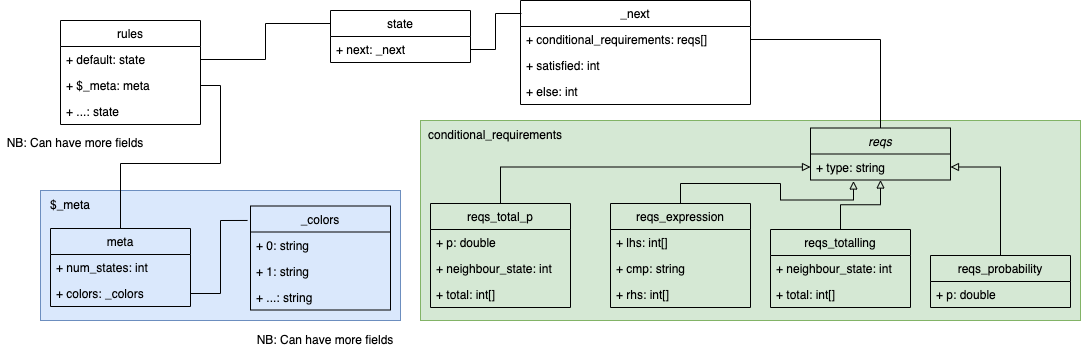
\includegraphics[scale=0.4]{uml_rules.png}
    \label{uml_rules}
\end{figure}

\noindent Overall, the reason of nesting the \texttt{conditional\_requirements}, \texttt{satisfied} and \texttt{else} keys in a \texttt{next} key after the state is mainly for code readability, particularly in the function builder, e.g. compare \texttt{json\_rules[0].satisfied} to \texttt{json\_rules[0].next.satisfied}. I argue the latter is more readable and verbose.

\newpage
\subsubsection{Examples of the Rules}
In order to grasp a better understanding of the rules, some examples are necessary. Their relationships are visualized in Figure \ref{uml_rules} above for reference. 
\\ \\
The general structure of the rules take the following form:
\\
\begin{center}
\begin{figure}[H]
\begin{verbatim}

                            {
                              $_meta: { ... },
                              default: { ... },      
                              0: { ... },
                              1: { ... },
                              ...
                            }
    
\end{verbatim}
\caption{General Structure of Rules}
\end{figure}
\end{center}
Note that the dots between the curly braces indicate a nested JSON object. The \texttt{\$\_meta} object only contains two key-value pairs. Below is an example of what the object may look like, and illustrates three valid ways of defining colors in the rules:
\begin{center}
\begin{figure}[H]
\begin{verbatim}
        
                            $_meta: {
                              num_states: 3,
                              colors: {
                                0: "red",
                                1: 255,
                                2: "#FF0000"
                              }
                            }
                
\end{verbatim}
\caption{Structure of \texttt{\$\_meta} object}
\end{figure}
\end{center}
As the previous section has stated, objects contained in the \texttt{default} key and any other numeric keys (0, 1, 2, etc.) contain the same structure. These objects are the \textbf{state transition rules}. In the following example, the \texttt{default} key contents will be shown:
\begin{center}
\begin{figure}[H]
\begin{verbatim}
        
                            default: {
                              next: {
                                conditional_requirements: [{ ... }],
                                satisfied: 1,
                                else: 0
                              }
                            }
                
\end{verbatim}
\caption{Structure of a basic state transition rule}
\end{figure}
\end{center}
The keys \texttt{satisfied} and \texttt{else} contain plain integers. The \texttt{conditional\_requirements} key contains a key of objects with the following formats:
\begin{center}
\begin{figure}[H]
\begin{verbatim}
        
                            conditional_requirements: [
                                {
                                  type: "totalling",
                                  neighbour_state: 1,
                                  total: [3],
                                }, 
                                {
                                  type: "probability",
                                  p: 1,
                                },
                                {
                                  type: "total-p",
                                  neighbour_state: 2,
                                  total: [1, 2, 3, 4],
                                  p: 0.8,
                                },
                                {
                                  type: "expression",
                                  lhs: {
                                    neighbour_states: [3, 4],
                                  },
                                  cmp: ">",
                                  rhs: {
                                    neighbour_states: [1, 2],
                                  },
                                }
                            ]
                
\end{verbatim}
\caption{Structure of conditional requirements list and different ways of specifying requirements}
\label{condreqslist_example}
\end{figure}
\end{center}
\noindent There are four ways of specifying a requirement for transition. And as shown in the Diagram in Figure \ref{uml_rules}, each variation of the requirements inherit the \texttt{type} parameter from its parent. For the above Figure \ref{condreqslist_example}, each requirement above can be translated to the following words in plain English, presented by the following table: 
\begin{table}[H]
\begin{tabular}{|l|l|}
\hline
\multicolumn{1}{|c|}{\textbf{Conditional Requirement}}                                                                                                                           & \multicolumn{1}{c|}{\textbf{Meaning}}                                                                      \\ \hline
\begin{tabular}[c]{@{}l@{}}\texttt{type: "totalling",}\\ \texttt{neighbour\_state: 1,}\\ \texttt{total: {[}3{]}}\end{tabular}                                                                              & There are a total of THREE neighbours with state ID 1                                                                        \\ \hline
\begin{tabular}[c]{@{}l@{}}\texttt{type: "probability",}\\ \texttt{p: 1}\end{tabular}                                                                                                             & There is a probability of 1                                                                                                  \\ \hline
\begin{tabular}[c]{@{}l@{}}\texttt{type: "total-p",}\\ \texttt{neighbour\_state: 2,}\\ \texttt{total: {[}1, 2, 3, 4{]},}\\ \texttt{p: 0.8}\end{tabular}                                                             & \begin{tabular}[c]{@{}l@{}}If there are 1, 2, 3, 4 neighbours with state ID 2, \\ there is a probability of 0.8\end{tabular} \\ \hline
\begin{tabular}[c]{@{}l@{}}\texttt{type: "expression",}\\ \texttt{lhs: \{}\\ \texttt{neighbour\_states: {[}3, 4{]},}\\ \},\\ \texttt{cmp: "\textgreater{}",}\\ \texttt{rhs: \{}\\ \texttt{neighbour\_states: {[}1, 2{]}} \\ \texttt{\}}\end{tabular} & If there are more of states 3 and 4 than 1 or 2                                                                              \\ \hline
\end{tabular}
\caption{Table of Interpretation from Rules to its meaning in English}
\label{rules_to_english_table}
\end{table}
\newpage
\subsection{Validator Component} \label{validator}
The Validator component is a standalone micro-component that compares the user-defined rules against the aforementioned JSON schema. Its functionality is called in the \\ \texttt{dynamic-rules-form.js} in validating the textarea's contents, in the form of the function \texttt{obeysJsonSchema()}. This component is an implementation of the TV4 library described in \ref{tv4}. 
\\ \\
The design choice of building the validator as the implementation of the TV4 library compared against a JSON schema is a practical choice done to save time. Developing an algorithm specific to this use case of iterating and testing the validity manually will require a great deal of time for research and implementation attempts. A general diagram on how the validator micro-component works is shown below:
\\
\begin{figure}[H]
    \caption{Validator Component Diagram}
    \centering
    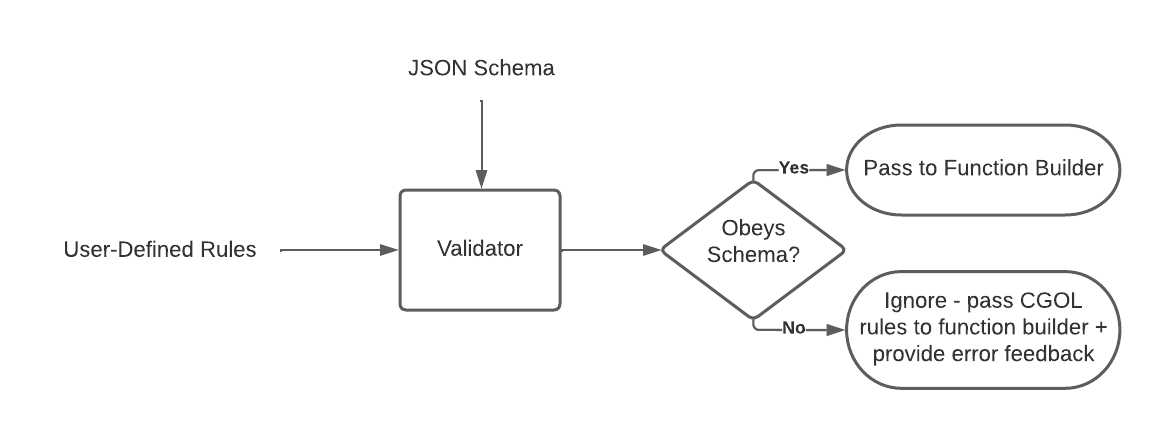
\includegraphics[scale=0.9]{validator_module.png}
\end{figure}
\noindent The validator attempts to determine the validity of rules passed to it in the system by parsing it (check to see if it's a valid JSON document), and the validity of it will be obtained by comparing against the provided JSON schema. Should the rules return invalid (or fail to parse), the validator will default to one of the system-default rules in the system, preventing the software to break.
\\ \\
The standalone \texttt{.js} file provided in the GitHub repository \ref{tv4} had a few integration problems such that the library was unable to use my supplied JSON schema \ref{json_schema} despite being able to use it online. That meant the simulator's validator had to use the Node Package variant of the library. 
\\ \\
The \textbf{Browserify} library was then used to compile the TV4 to yet another standalone \texttt{.js } file so it can provide support for browser applications \cite{browserify}.
\newpage

\subsection{Function Builder} \label{f_builder}
The function builder will accept values approved by the validator. This will either be one of the system's default rules, or the valid user-defined rules provided from the rule editor. CA rules have the capability of being defined by conditional statements (i.e. if-else statements). The pipeline of the function creator component will consist of parsing the given \texttt{conditional\_requirements} from the provided rules into if-statements, and then passed as an anonymous function to be used as the simulator's transition rules. 
\\ \\
The design of each the components making up the function builder component will now be described in the following subsections. This component and other micro-components contained can be found in the \texttt{function-builder.js} file in the \texttt{utils} folder. 
\\ \\
Overall, there are three major micro-components of the function builder: that is the condition builder, the if-statement builder, and the anonymous function builder. The architectural diagram for this module's running is provided as below:
\\
\begin{figure}[H]
    \caption{Function Builder Component and Micro Components}
    \centering
    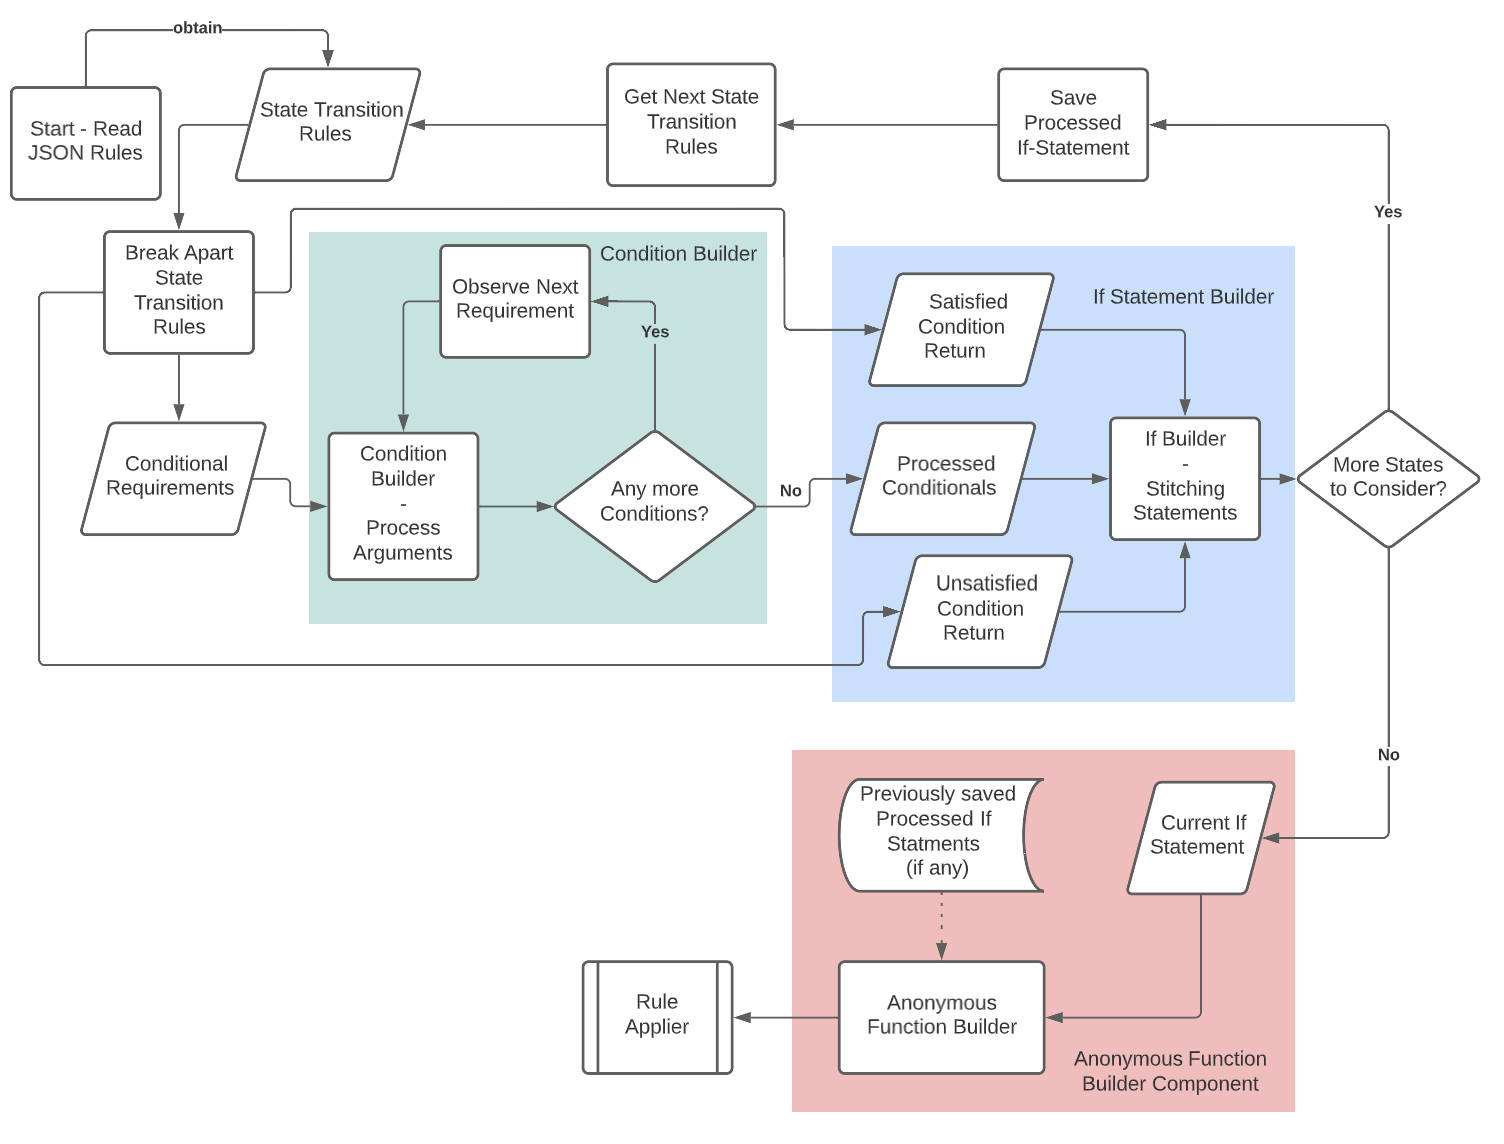
\includegraphics[scale=0.70]{functionbuilder_module.png}
\end{figure}
\subsubsection{Condition Builder}
I define conditions in this project as the values that are placed inside an if-statement. The condition builder is a micro-component within the function builder component that processes the inner most values of the rules from the format, i.e. the \texttt{conditional\_requirements} list. As described in section \ref{rules_format} on the rules format, the condition builder builds four types of conditions. 
\\ \\
Referring to Table \ref{rules_to_english_table}, the conditional requirements are translated into the following conditions in the following format:
\begin{table}[H]
\begin{tabular}{|l|l|}
\hline
\multicolumn{1}{|c|}{\textbf{Conditional Requirement}}                                                                                                                           & \multicolumn{1}{c|}{\textbf{Resulting Conditional}}                                                                      \\ \hline
\begin{tabular}[c]{@{}l@{}}\texttt{type: "totalling",}\\ \texttt{neighbour\_state: 1,}\\ \texttt{total: {[}3{]}}\end{tabular}                                                                              & \texttt{[3].includes[neighbours[1]]}                                                                        \\ \hline
\begin{tabular}[c]{@{}l@{}}\texttt{type: "probability",}\\ \texttt{p: 1}\end{tabular}                                                                                                             & \texttt{probability(1)}                                                                                               \\ \hline
\begin{tabular}[c]{@{}l@{}}\texttt{type: "total-p",}\\ \texttt{neighbour\_state: 2,}\\ \texttt{total: {[}1, 2, 3, 4{]},}\\ \texttt{p: 0.8}\end{tabular}                                                             & \begin{tabular}[c]{@{}l@{}} \texttt{(probability(0.8) \&\&} \\ \texttt{[1,2,3,4].includes(neighbours[2])} \end{tabular} \\ \hline
\begin{tabular}[c]{@{}l@{}}\texttt{type: "expression",}\\ \texttt{lhs: \{}\\ \texttt{neighbour\_states: {[}3, 4{]},}\\ \},\\ \texttt{cmp: "\textgreater{}",}\\ \texttt{rhs: \{}\\ \texttt{neighbour\_states: {[}1, 2{]}} \\ \texttt{\}}\end{tabular} & \texttt{neigh[3] + neigh[4] \textgreater{} neigh[1] + neigh[2]}                                                                    \\ \hline
\end{tabular}
\caption{Translation Table from Rules to JS Conditions Implementation}
\label{rules_to_english_table}
\end{table}
\noindent Important to note that \texttt{neigh} is the same as \texttt{neighbours} and are dictionaries. They are defined in Section \ref{ncrc} and are allocated every cell. In essence, \texttt{neighbours[1]} holds the amount of type \texttt{1} neighbours the cell in test has.
\\ \\
When there are multiple conditional requirements provided in the list, then the conditionals are connected via an \texttt{OR} connection. There was no specific reason in choosing to connect the conditionals with an \texttt{OR} instead of \texttt{AND}, apart from the fact that configuring the connectives could be a feature to be added another day.

\subsubsection{Probability Calculator (Micro Component)} \label{prob_calc_fbuilder}
The probability calculator micro component complements the functionality of the condition builder. Its purpose is defined above in number \ref{probability_condreq} of the \texttt{type} key value of the \\ \texttt{conditional\_requirement} object. Its evaluation, however, is called in the Actuator component. That being said, it is not shown in the diagram. Its overall usage is described in the \ref{actuator} subsection below.

\subsubsection{If Builder}
The If Builder is a straightforward micro-component that accepts values (conditions) passed from the condition builders. It takes two integer arguments (\texttt{satisfied\_rtn} and \texttt{otherwise}) for the states to transition to, and a string argument \texttt{conditions}. This micro-component simply returns a literal string value of the built if statement.

\subsubsection{Anonymous Function Generator}
Once the rules are read and the appropriate micro-components are utilized, the final part of the function builder relies on a JS anonymous function builder. The anonymous functions are then passed to the actuator, where the rules are ultimately applied in the simulator.

\subsection{Actuator} \label{actuator}
The actuator will function as the simulator's back-end. Two major functionalities of the actuator is counting the Moore Neighbours of each cell in the CA and applying the rules supplied by the function builder. These functionalities are triggered by the buttons. Additionally, the actuator is the first component that is called to action in the system as it renders the entire page as the \texttt{setup()} function is executed in the \texttt{sketch.js} file. The \texttt{setup()} function operates quite trivially as it only assigns the default starting variables, and it therefore won't be discussed here. 
\subsubsection{Initializer} \label{initializer}
The initializer is a micro-component for the actuator. It is the first part of the actuator that is called when a user accesses the tool, or make changes to the rules and system. More importantly, the initializer renders the front end. This component is therefore both a back-end and a front-end component. In essence, the initializer determines the following variables:
\begin{itemize}
    \item \textbf{Number of States}: This variable is supplied to a variety of components, i.e. the color allocator micro component (see \ref{color_allocator})
    \item \textbf{Active Rules}: The active rules are the transition rules for the simulator, after the approval from the validator component (see \ref{validator}) and processed by the function builder (see \ref{f_builder}). 
    \item \textbf{2D Array Dimensions}: These dimensions (rows and columns) are determined in this setup. These values are passed on to the respective 2D Array Creator (see subsection below).
\end{itemize}

\subsubsection{Two-Dimensional Array Creator (Micro Component)} \label{2darr_creator}
As the heading suggests, the actuator contains a two-dimensional array creator. This functionality is used by the initializer (see above) and by the Rule Applier micro component within this component (see \ref{ncrc}). Two-dimensional arrays are used as the CA simulator two-dimensional grid, thus emphasizing its importance. 
\\ \\
Rows and Columns of this two-dimensional array are calculated by dividing the width and height of the user's screen with the resolution.
\newpage
\subsubsection{Color Allocator (Micro Component)} \label{color_allocator}
The color allocator is a micro component within the actuator that focuses on color allocation for each state. In essence, it returns an Array whose indexes correspond to the state number, and the contents contained at the index is the state's color. For example, consider a five-state CA with states labelled from 0-4:
\begin{figure}[H]
    \caption{State Number Corresponding to Color}
    \centering
    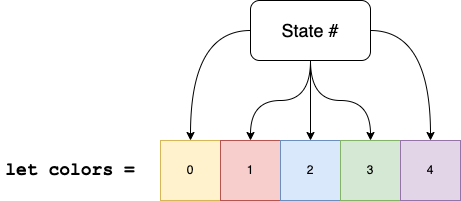
\includegraphics[scale=0.50]{aoc.png}
\end{figure}
\noindent The color of State \# 0 is therefore contained in \texttt{colors[0]} (yellow), State \# 1 in \texttt{colors[1]}, and so on. The color of state \# k is contained in \texttt{colors[k]}.
\\ \\
The allocator firstly checks whether the \texttt{colors} key exists in the \texttt{\$\_meta} object and if the number of states are equal to the number of keys contained in \texttt{colors}, and they values contained in the keys are of valid color representations. Otherwise, random colors are allocated to the states. The flowchart of this micro-component can be seen below:
\\
\begin{figure}[H]
    \caption{Color Allocator Flowchart}
    \centering
    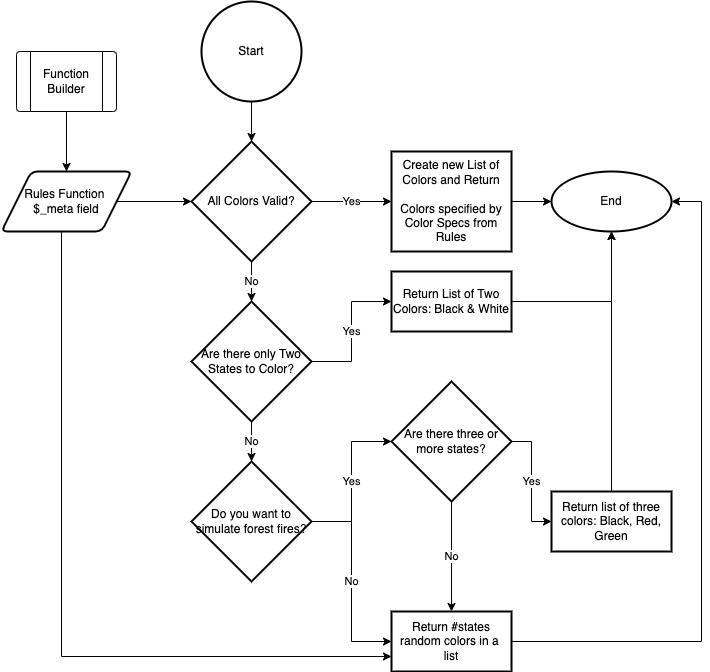
\includegraphics[scale=0.45]{flowchart_coloralloc.drawio.png}
\end{figure}
\newpage
\subsubsection{Actuator Buttons}
The buttons (seen in the top part of figure \ref{fig:final_gui}) serve as the inputs (operating similarly to remote) to the actuator. Though the buttons are essentially rendered as part of the GUI, its main functionality is defined in the actuator class. The following buttons are provided, and their actions:
\begin{itemize}
    \item Play/Pause: 
    There is a \texttt{pause} variable of type \texttt{boolean} in the system that drives whether the simulator should execute or not. While \texttt{pause} is initially set to \textit{True}, this button negates the value of \texttt{pause}, where there is another function \texttt{draw()} essentially runs the simulator. 
    \item Single Step: 
    The single step button operates the same way as the play/pause button, but what this button does in a single run is explicitly declare \texttt{pause} to \textit{True}, calls the \texttt{draw()} function, and then resets \texttt{pause} to \textit{False}
    \item Randomize:
    The randomize button essentially creates a new two-dimensional array according to the number of states and associated number of If colors are not provided to each state from the \texttt{\$\_meta} tag, then they are randomly allocated by the color allocation micro-component above in section \ref{color_allocator}.
\end{itemize}
The flowcharts for the buttons are shown below:
\\
\begin{figure}[H]
    \caption{Button Actions Flowchart}
    \centering
    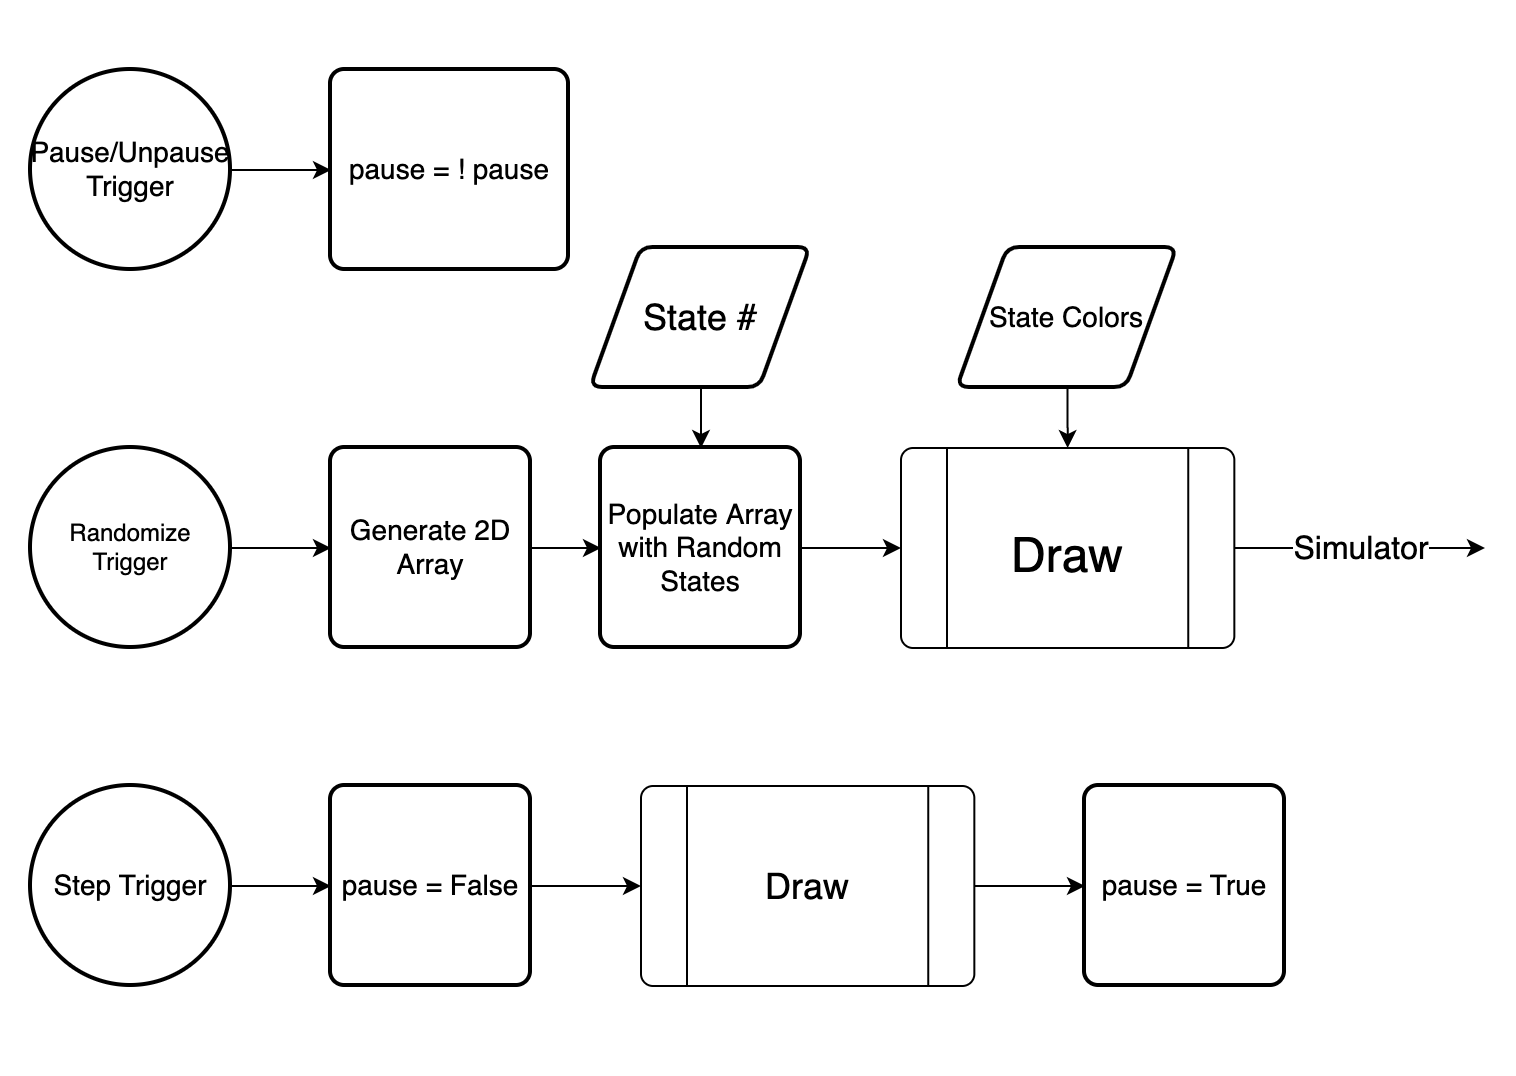
\includegraphics[scale=0.50]{buttonactions_module.png}
\end{figure}

\newpage
\subsubsection{Neighbour Counter \& Rule Applier} \label{ncrc}
CAs commonly consider the neighbour numbers and states before deciding what to do next. That being said, neighbour numbers and their states are typically calculated in one single function, that is when the rules are applied. However, integrating both functionalities into a single micro-component introduces a higher level of cognitive complexity in the algorithms, making it potentially harder to manage, and maybe even add features.
\\ \\
For that reason, these micro-components are separately defined (in different functions) for modularity. However, in the running process of the rule applier micro-component, it calls the function of the neighbour counter. Following is the flowchart of the Rule Applier:
\\
\begin{figure}[h]
    \caption{Rule Applier Flowchart}
    \centering
    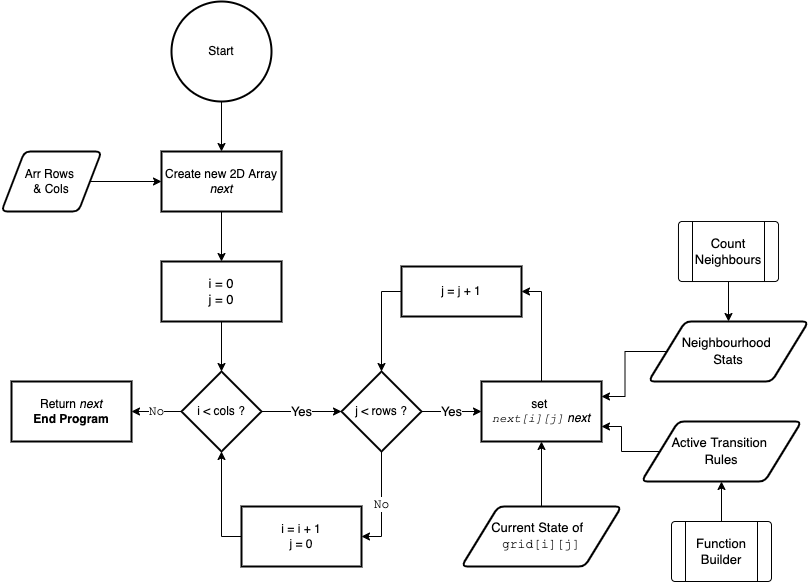
\includegraphics[scale=0.50]{ruleapplier.drawio.png}
\end{figure}
\\
The rule applier essentially creates a new two dimensional array of cells with the same dimensions as the current grid, iterates each cell from top left to bottom right by using a nested for-loop, assigning new states to the cells at the new array (with input from neighbour count and cell's current state). 
\newpage
\noindent The neighbour counter operates as specified by the following chart:
\begin{figure}[H]
    \caption{Neighbour Counter Flowchart}
    \centering
    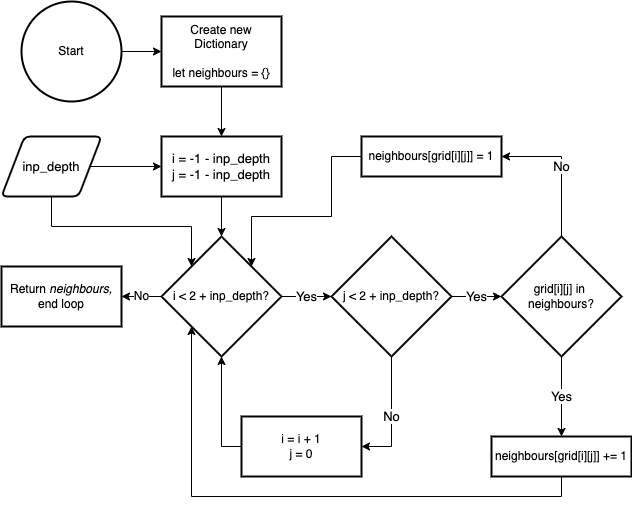
\includegraphics[scale=0.50]{flowchart_neighbourcounter.png}
\end{figure}

\noindent The design choice of implementing an infinite two-dimensional grid (instead of a finite grid in the provided frame) was made due to the fact that CAs are typically based on an infinite grid, particularly CGOL \cite{kier2005modeling}. The way this was implemented is reflected in the rule applier code, where the cells wrap around each other (e.g. bottom right cell's neighbour includes top left cell, and vice versa).
\newpage
\subsection{Sketcher}
The sketcher (or simulator) visualizes the current CA grid and its colors. This component has mostly stayed the same in the context of its GUI appearance, and is purely front end. It accepts two dimensional arrays containing the new state of the CA. This component utilizes the P5JS library, described in \ref{p5js}. A small part of the sketching process occurs in the highlighted area in the flowchart below:
\\
\begin{figure}[H]
    \caption{Flowchart of Sketcher}
    \centering
    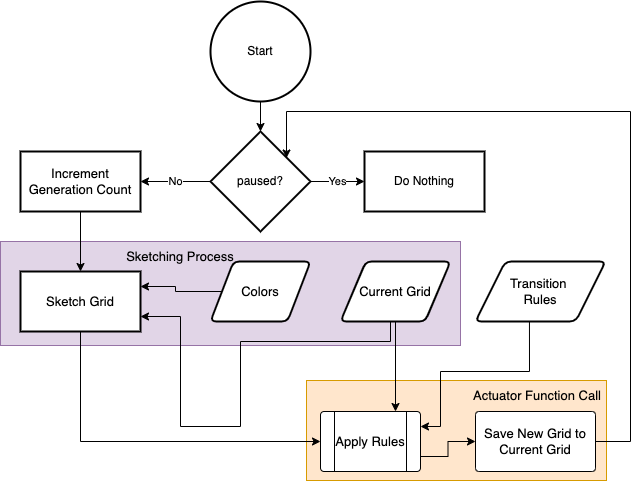
\includegraphics[scale=0.50]{flowchart_sketcher.png}
\end{figure}
\noindent The \texttt{sketch()} function attempts to visualize the CAs in the simulator. Additionally, this module calls the functionality of the actuator (indicated as well in the flowchart) to keep its process running.

\subsection{Help Page}
Finally, there is a basic help page that is essentially a static \texttt{.html} page. It describes the basics of CAs. Additionally, this page outlines a basic tutorial on how to use the tool, and more importantly learn the proper syntax of the rules to input to the system through the editor. As this component is a simple HTML page, no component diagram is specified, nor will this be represented in the general architectural diagram. 
\\ \\
The help page can be accessed through a button above the rules editor.
\newpage
\section{Dependency Graph}
This graph shows the dependencies needed by each of the written components in order to properly function. Arrows from component \textbf{A} pointing towards another component \textbf{B} signify that "component \textbf{A} depends on component \textbf{B}". Additionally, the external libraries are highlighted in the diagram.
\\
\begin{figure}[h]
    \caption{Dependency Diagram}
    \centering
    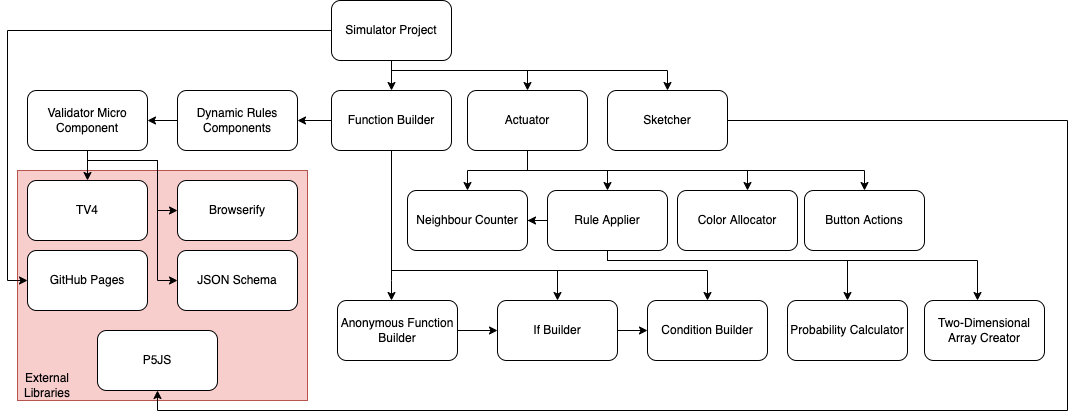
\includegraphics[scale=0.45]{dependency_diagram2.png}
\end{figure}
\\
Note that some component names were not listed such as the GUI (see \ref{gui_component}) and the Initializer (see \ref{initializer}) as their functionalities are purely front end. Inherently, they depend on each and every one of the components and form as part of the simulator project itself. 